\documentclass[a4paper,12pt]{report}
\usepackage{alltt, fancyvrb, url}
\usepackage{graphicx}
\usepackage[utf8]{inputenc}
\usepackage{float}
\usepackage{hyperref}
\usepackage{minted}
\usepackage{tcolorbox}

\newcommand{\myexample}[2]{
    \begin{tcolorbox}[colback=black!5!white,colframe=black,title={Esempio: #1}]
        #2
    \end{tcolorbox}
}
\graphicspath{{./images}}

% Questo commentalo se vuoi scrivere in inglese.
\usepackage[italian]{babel}

\usepackage[italian]{cleveref}
\title{Relazione del progetto di Programmazione di Reti 
    \\ Traccia 1: Configurazione di una Rete con VLAN e Routing Inter-VLAN}

\author{Leonardo Grimaldi}
\date{\today}   
\begin{document}
\maketitle
\tableofcontents
\chapter{Consegna}
\section{Descrizione}
Gli studenti dovranno progettare e configurare una rete che include due LAN separate in due VLAN su GNS3, utilizzando switch e router virtuali. La configurazione richiederà il routing inter-VLAN per permettere la comunicazione tra le VLAN.
\section{Obiettivi}
Configurare VLAN, routing inter-VLAN, e verificare la connettività tra dispositivi su VLAN diverse.
\section{Consegne richieste}
Documentazione della configurazione, spiegazione dei comandi utilizzati e cattura del traffico di rete per dimostrare la comunicazione tra le VLAN.
\chapter{Progettazione}
I due campus dell'Università di Bologna, il Campus di Cesena e il Campus di Bologna sono costituiti da due dipartimenti: IT (Information Technology) e di ricerca.
%
Essi possiedono due edge router che possono scambiarsi informazioni per mezzo di una WAN (Wide Area Network), semplificato con un collegamento diretto.
%
Il traffico dei dipartimenti all'interno del singolo Campus vuole essere separato, mentre si vuole consentire la comunicazione inter-dipartimentale tra i due Campus.
%
\myexample{Ping tra i Campus}{
    Scientifico Cesena Scientifico Bologna
    %
    Scientifico Cesena  IT Bologna
}
La topologia di rete è proposta nella figura \ref{fig:topologia_offline}. 
\begin{figure}
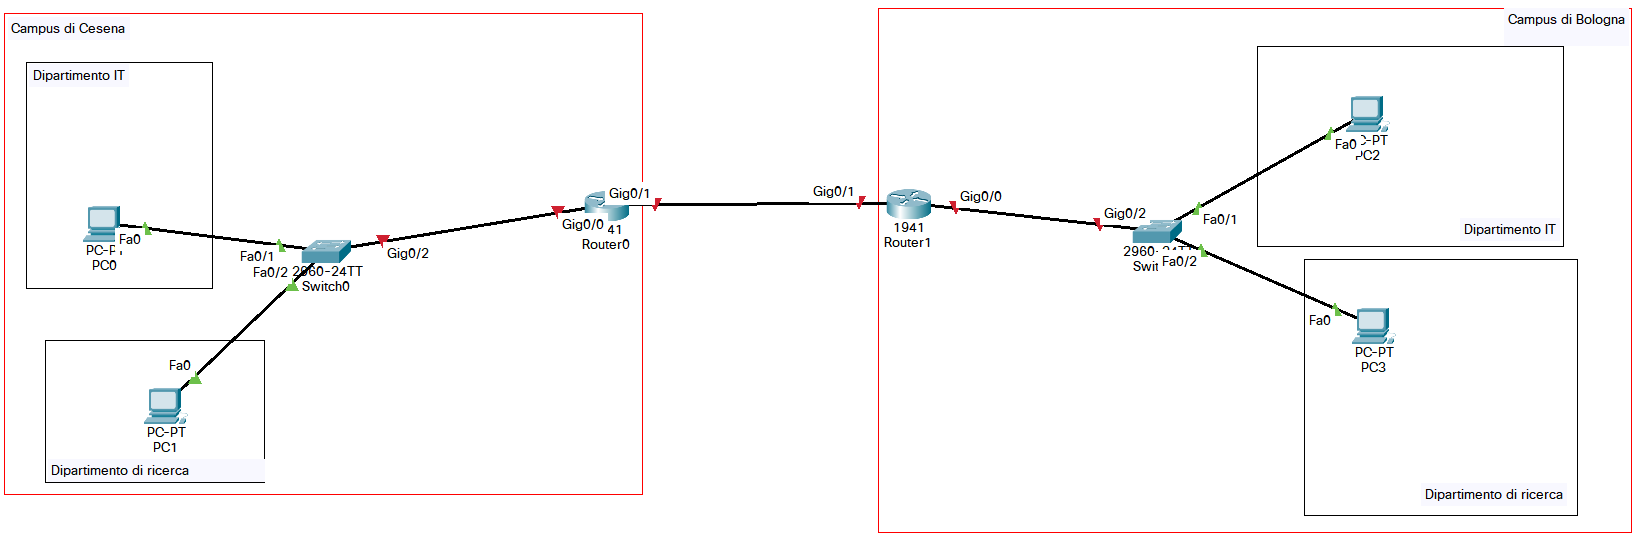
\includegraphics[width=\textwidth]{offline_topology_with_departments.png}
\caption{
    Topologia di rete dei dipartimenti di IT e ricerca tra il Campus di Cesena e Bologna.
    %
    I triangolini rossi sui collegamenti indicano che il link è offline.
    }
\label{fig:topologia_offline}
\end{figure}
\chapter{Configurazione}
Partendo dalla configurazione interna al Campus, è necessario stabilire gli indirizzi IP per i computer e per l'interfaccia router.

\end{document}